%% -*- eval: (flyspell-mode 1); -*-

\chapter{\'Evaluation de la bibliothèque}

Le DSEL doit être évalué dans plusieurs domaines : à la fois en matière d'expressivité du langage et à la fois du point de vue des performances matérielles (la rapidité d'exécution). Ces deux évaluations ont été difficiles à réaliser car d'une part l'expressivité est difficilement quantifiable, et d'autre part car le DSEL s'appuie sur la bibliothèque \textsf{triSYCL} qui est seulement un prototype -- une preuve de concept également.


\section{\'Evaluation qualitative}

La qualité du DSEL peut se juger à la facilité d'écriture de code l'utilisant. Globalement il faudrait alors évaluer à quel point la librairie permet d'abstraire le problème qu'elle est censée résoudre (ici la parallélisation de stencils). Plus particulièrement il s'agit de quantifier notamment du pseudo-typage (erreurs sémantiques statiques), du nombre de mots-clés (classes, méthodes), du nombre de symboles, et enfin du nombre de lignes de codes (LOC). Pour des raisons de simplicité seul le nombre de ligne de codes ainsi que le nombre de caractères ont été pris en compte. 

Ces deux nombres ont été comparé entre plusieurs codes d'un même problème de Jacobi en deux dimensions avec un stencil à cinq points. Les différentes versions du code sont :
\begin{enumerate}
\item code de base sans parallélisation ;
\item code \textsf{OpenMP} avec parallélisation naïve ;
\item code \textsf{OpenMP} avec parallélisation par tuilage ;
\item code \textsf{triSYCL} avec parallélisation naïve ;
\item code \textsf{triSYCL} avec parallélisation par tuilage ;
\item code \textsf{DSEL} avec parallélisation et coefficients variables ;
\item code \textsf{DSEL} avec parallélisation et coefficients constants ;
\item code \textsf{OpenCL} avec parallélisation par tuilage.
\end{enumerate}

Les deux versions du DSEL ne se déclinent pas en parallélisation avec tuilage ou naïve puisque celle-ci est simplement choisie par l'appel d'une méthode ou l'autre, dont les noms ne différent que de cinq caractères (qui ont été comptabilisés). Par ailleurs pour comptabiliser les lignes de codes et caractères, toutes les lignes vides n'ont pas été comptabilisées, de même que les commentaires. De plus les conventions de codage (pour les retours à la ligne et la disposition des arguments) sont les mêmes pour les $8$ codes. Enfin aucune entrée/sortie standard (en dehors des erreurs) n'est intégrée dans le décompte des deux métriques ; les seules erreurs reportées se trouvent dans le code d'\textsf{OpenCL}, car c'est à la charge de l'utilisateur de les traiter contrairement aux autres codes (\textsf{OpenMP} n'en n'a pas besoin dans ce cas, et celles de \textsf{triSYCL} sont gérées en interne de même que le DSEL qui s'appuie sur \textsf{triSYCL}).

Les résultats sont reproduits dans le tableau \ref{tab:eval_qual} où l'on peut observer que le DSEL (avec coefficients constants) est le troisième code le plus court avec $42$ lignes, tandis que le plus court (code de base) en comporte $31$. Le DSEL avec coefficients constants se classe cinquième avec $46$ lignes. En ce qui concerne les codes avec tuilage, ils ont deux fois (\textsf{OpenMP}) à cinq fois (\textsf{OpenCL}) plus long que le code de base. Le classement est quasiment identique selon le nombre de caractères (à une inversion près, ne concernant pas le DSEL).

\begin{table}
\floatbox[{\capbeside\thisfloatsetup{capbesideposition={right,center},capbesidewidth=4cm}}]{table}[\FBwidth]
{
\caption{Évaluation du nombre de lignes de codes et de caractères pour différentes implantations d'un problème Jacobi2D.}
\label{tab:eval_qual}
}
{
\begin{tabular}{||c||c|c||}
\hline
implantation & LOCs & caractères \\
\hline
\hline
base & $31$ & $899$ \\
\hline
OpenMP naïf & $32$ & $924$ \\
\hline
OpenMP tuilage & $87$ & $3115$ \\
\hline
triSYCL naïf & $43$ & $1676$ \\
\hline
triSYCL tuilage & $74$ & $3647$ \\
\hline
DSEL variable & $46$ & $1919$ \\
\hline
DSEL constant & $42$ & $1624$ \\
\hline
OpenCL tuilage & $177$ & $6266$ \\
\hline
\end{tabular}
}
\end{table}

En résumé, l'écriture du code grâce au DSEL est du même ordre de grandeur que l'écriture des codes parallélisés naïfs (à quelques lignes près) lors qu'il propose l'optimisation de tuilage. Les autres codes proposant le tuilage étant quant à eux deux à cinq fois plus longs que le code de base, le DSEL permet ainsi une amélioration significative des performances (grâce au tuilage) sans augmenter substantiellement la charge de développement (estimée en LOCs).


\section{Performances quantitatives sur machines dédiées}

Les performances quantitatives s'appuient sur deux métriques : le temps d'exécution et les compteurs \emph{hardwares}. Tandis que la rapidité d'exécution est l'objectif principal de la librairie, les compteurs permettent de comptabiliser indirectement la réutilisation des données, qui plus elle est grande plus elle favorise la rapidité. Le protocole de tests est présenté en premier, avant de préciser plus en détail les résultats de ces mesures.

\subsection{Description du matériel et des cas de tests}
\label{sec:desc_mat_tests}

L'optimisation de calculs faisant intervenir de nombreux paramètres, plusieurs implantations et machines différentes ont été utilisées. Le protocole de test consiste à exécuter chacune des implantations deux ou trois fois de suite (selon les machines) pour un même jeu de paramètres, puis de faire varier ces paramètres et recommencer. C'est la moyenne des résultats des deux ou trois exécutions de chaque cas de test qui est ici analysée, ce faible nombre d'exécution est suffisant puisque les premières mesures manuelles n'ont révélées que des différence inférieures à $1\%$. Par ailleurs chaque implantation applique trois fois le stencil d'affilée, les résultats des mesures de chacune des trois applications sont simplement sommés formant alors le résultat utilisé pour calculer la moyenne.

\subsubsection*{Implantations testées}

Afin de pouvoir évaluer certains paramètres pouvant influencer les performances, il a été nécessaire de ne pas utiliser directement le DSEL produit mais uniquement la bibliothèque \textsf{triSYCL} de parallélisation sur laquelle il s'appuie ainsi que \textsf{OpenMP} (utilisée par \textsf{triSYCL}). Toutefois cela n'a pas d'impact sur les performances, car les implantations ont été écrites dans l'esprit du code automatique produit par le DSEL. De plus les méthodes du DSEL sont marquées pour être \emph{inlinées} dans le code d'origine, et ne provoquent donc pas d'appels supplémentaires dans l'exécution du programme. Ainsi nous pouvons considérer que les performances mesurées sont équivalentes à celles du DSEL.

Ne pas utiliser directement le DSEL permet notamment de modifier artificiellement le coût du calcul d'un élément de la grille dans le problème de Jacobi en deux dimensions. En effet chaque élément de la grille est dupliqué un certain nombre de fois (paramètre variable), la charge de calcul est donc dupliquée autant de fois. En pratique chaque élément représente donc une \emph{tuile} dont tous les sous-éléments sont identiques. L'application d'un coefficient sur un élément correspond alors à la multiplication matricielle de la tuile (qui est un vecteur à une seule dimension) par une matrice identité dont la diagonale a la valeur du coefficient originel. Moduler le coût du calcul d'un élément permet à la fois de modifier sa durée, et aussi la quantité de mémoire qu'il utilise puisque l'élément est dupliqué.

Afin de vérifier que l'implantation elle-même est valide, une validation automatique des résultats a été réalisée dans le problème d'origine, sans tuiles. En revanche les implantations évaluées dont les résultats sont présentés dans les sections suivantes ne concernent que des implantations avec tuiles. Elles ne nécessitent que quelques lignes de code supplémentaires mais ralentissent énormément la vérification des résultats (puisque chaque élément est dupliqué un certain nombre de fois) ; ainsi seule une vérification manuelle a été faite sur des petits jeux de données. Par ailleurs l'application du stencil est volontairement divergente afin de pouvoir distinguer les valeurs des éléments avant et après l'application du stencil. Ces vérifications n'ont pas permis de détecter une erreur significative (à $1^{-06}$ près) entre les différentes implantations, que nous considérons donc valides. 

Seuls deux paramètres de tests ont été étudiés :
\begin{itemize}
\item la taille de chaque macro-tuile carrée ;
\item la taille de chaque tuile.
\end{itemize}
Les autres paramètres n'ont pas été étudiés soit par manque de temps, soit parce qu'il n'avait pas d'influence a priori telle que la taille globale du système que nous supposons toujours inférieure à la taille de la RAM.

Ces deux paramètres peuvent alors influencer le comportement des implantations suivantes testées :
\begin{enumerate}
\item parallélisation naïve par \textsf{OpenMP} ;
\item parallélisation naïve par \textsf{triSYCL} (qui s'appuie sur \textsf{OpenMP}) ;
\item parallélisation par tuilage avec \textsf{OpenMP} ;
%% \item parallélisation par tuilage en column major avec \textsf{OpenMP} ;
\item parallélisation par tuilage avec \textsf{OpenMP}, représentation des macro-tuiles continue en mémoire RAM ;
\item parallélisation par tuilage avec \textsf{OpenMP}, parallélisme hiérarchique ;
\item parallélisation par tuilage avec \textsf{triSYCL}.
\end{enumerate}
Les codes $1$, $2$ s'appuient sur la découpe des boucles \textsf{for} de plus bas niveau en autant de section distinctes et parallèles qu'il y a de cœurs disponibles. Les codes $3$, $4$ et $6$ reprennent la technique de parallélisation par tuilage, à la différence près qu'il y a plus d'éléments par macro-tuile qu'il y a de cœurs. Les calculs y sont donc effectués par tâche : dès qu'un cœeur a fini sa tâche (l'application du stencil sur un élément), il passe à la suivante jusqu'à ce qu'il y en ait plus. Enfin le code $5$ crée également des tâches mais qui correspondent cette fois chacune au calcul d'une macro-tuile entière. Ces \emph{macro-tâches} sont alors calculées par chaque banc NUMA de la machine, et chaque macro-tuile est parallélisée naïvement comme pour les codes $1$ et $2$ au sein d'un banc NUMA.

Enfin plusieurs variantes de ces implantations ont été étudiées :
\begin{itemize}
\item exécution séquentielle, parallèle ou via support d'exécution ;
\item allocation par \textsf{malloc} ou par \textsf{boost} (pour les implantations avec \textsf{triSYCL}) ;
\item initialisation de la grille dans le même ordre que les calculs ou non ;
\item recopie des données (puisque le calcul n'est pas fait en place) avec tuilage ou non (pour les implantations par tuilage).
\end{itemize}


\subsubsection*{Machines de tests}

Les machines de tests utilisées sont celles disponibles sur \textsf{PlaFRIM}, le supercalculateur du campus de Bordeaux partagé entre différents laboratoires de recherche. Plus particulièrement nous avons utilisé les machines \textsf{Manumanu}, \textsf{Fourmi} et \textsf{Mistral}. Leurs caractéristiques techniques sont détaillées dans le tableau \ref{tab:carac_mach}.

\begin{table}
{
\caption{Caractéristiques des machines utilisées sur \textsf{PlaFRIM}.}
\label{tab:carac_mach}
}
{
\begin{tabular}{||c||c|c|c|c|c||}
\hline
Machine & Bancs NUMA & Cœurs par banc & Processeur\\% & Cache L3 & Cache L1 \\
\hline
\hline
Manumanu & $20$ & $8$ & Xeon E7-8837 @2.67 GHz \\% & $24$ MB & $256$ KB \\
Fourmi & $2$ & $4$ & Nehalem Xeon X5550 @2.66 GHz \\% & $8192$ KB & $256$ KB \\
Mistral & $2$ & $10$ & Ivy-Bridge Xeon E5-2670v2 @2.50 GHz \\% & $25$ MB & $256$ KB \\
\hline
\end{tabular}
}
\end{table} 

Par ailleurs les compilateurs utilisés sur ces machines sont \textsf{g++ 4.9.2} pour \textsf{Manmanu} et \textsf{Mistral}, et \textsf{g++ 4.9.0} pour \textsf{Fourmi}. Ils utilisent tous la version associée d'\textsf{OpenMP}, ainsi que \textsf{boost 1.58} (pour \textsf{triSYCL}).

Ces machines n'ayant pas les mêmes caractéristiques, les optimisations à réaliser et tester ne sont pas les mêmes. L'optimisation des caches a notamment été évoquée à la section \ref{sec:obj_perf} : il s'agit de faire rentrer la mémoire utilisée par le calcul d'une macro-tuile dans le cache L3, et la mémoire utilisée par un élément dans le cache L2. La solution optimale à ses deux problèmes peut être calculée de manière exacte par la résolution de deux équations linéaires du second degré. En effet notons $x$ la taille d'une tuile et $y$ la taille d'une macro-tuile (carrée), ainsi que $a$ la taille du cache L2, et $b$ la taille du cache L3. Dans le cas de problème de Jacobi à deux dimensions, la mémoire utilisée par un cœur correspond d'après les implantations utilisées à $7$ tuiles ainsi que la matrice de coefficients. En ce qui concerne l'ensemble des cœurss, au nombre de $c$ qui partagent le même cache L3 (même banc NUMA), ils stockent la matrice de coefficients ainsi que $7 \times c$ tuiles (les caches L3 sont inclusifs) et une macro-tuile entière. Il est donc possible de calculer la taille optimale d'une tuile pour le cache L1 puis d'utiliser cette taille pour calculer la taille optimale d'une macro-tuile pour le cache L3. Enfin précisons que les calculs sont effectués avec le type \textsf{float} qui utilisent $4$ Bytes. Ainsi nous obtenons l'équation \ref{eq:cache_L2} pour le cache L2 et \ref{eq:cache_L3} pour le cache L3.

\begin{equation}
\label{eq:cache_L2}
4x^2 + 4x \times 7 \leq a
\end{equation}

\begin{equation}
\label{eq:cache_L3}
4x^2 + c \times 4x \times 7 + y^2 \times 4x \leq b
\end{equation}

Compte-tenu de ces équations et des tailles de caches des machines utilisées, les résultats sont présentés dans la table \ref{tab:size_cach}. Les équations n'ayant pas de solutions entières, nous avons choisi la solution étant une puissance de deux immédiatement inférieure à la solution positive maximale.

\begin{table}
{
\caption{Tailles optimales (et solutions réelles positives) des tuiles et macro-tuiles pour les machines de \textsf{PlaFRIM}.}
\label{tab:size_cach}
}
{
\begin{tabular}{||c||c|c|c|c|c||}
\hline
Machine & Taille tuile & Taille macro-tuile & Cache L3 & Cache L1 \\
\hline
\hline
Manumanu & $128$ ($252.52$) & $128$ ($221.29$) & $24$ MB & $256$ KB \\
Fourmi & $128$ ($252.52$) & $64$ ($127.39$) & $8192$ KB & $256$ KB \\
Mistral & $128$ ($252.52$) & $128$ ($225.84$) & $25$ MB & $256$ KB \\
\hline
\end{tabular}
}
\end{table} 


\subsection{Mesures de temps et compteurs}

(Pour hiérarchisation, \cite{Ths3,Ths4})

\begin{figure}[!h]
  \caption{Comparaison des performances en temps suivant la taille des tuiles et des macro-tuiles.}
  \label{graph:comp_tuile_time}
  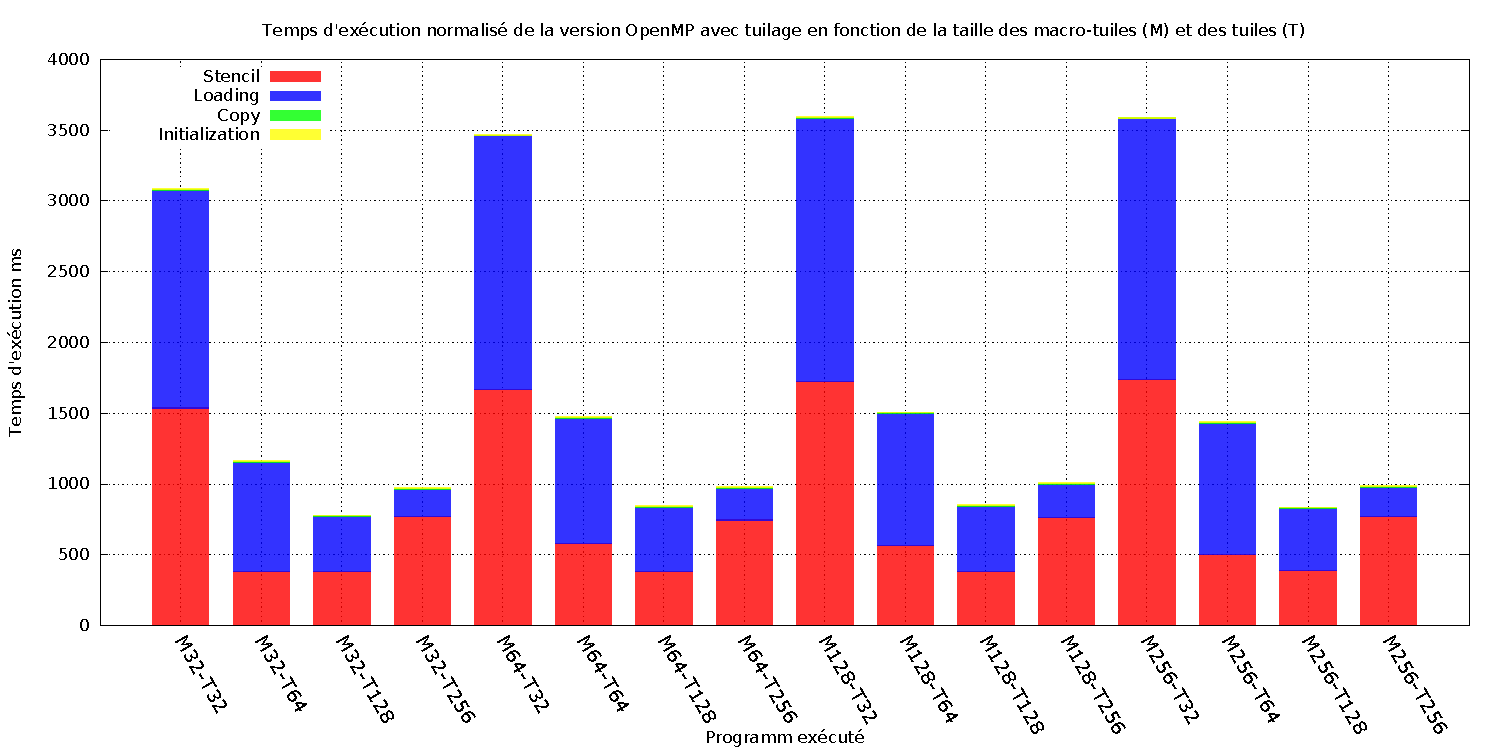
\includegraphics[width=\textwidth]{graph1.pdf}
\end{figure}

\begin{figure}[!h]
  \caption{Comparaison des performances en compteurs matériels suivant la taille des tuiles et des macro-tuiles.}
  \label{graph:comp_tuile_cmiss}
  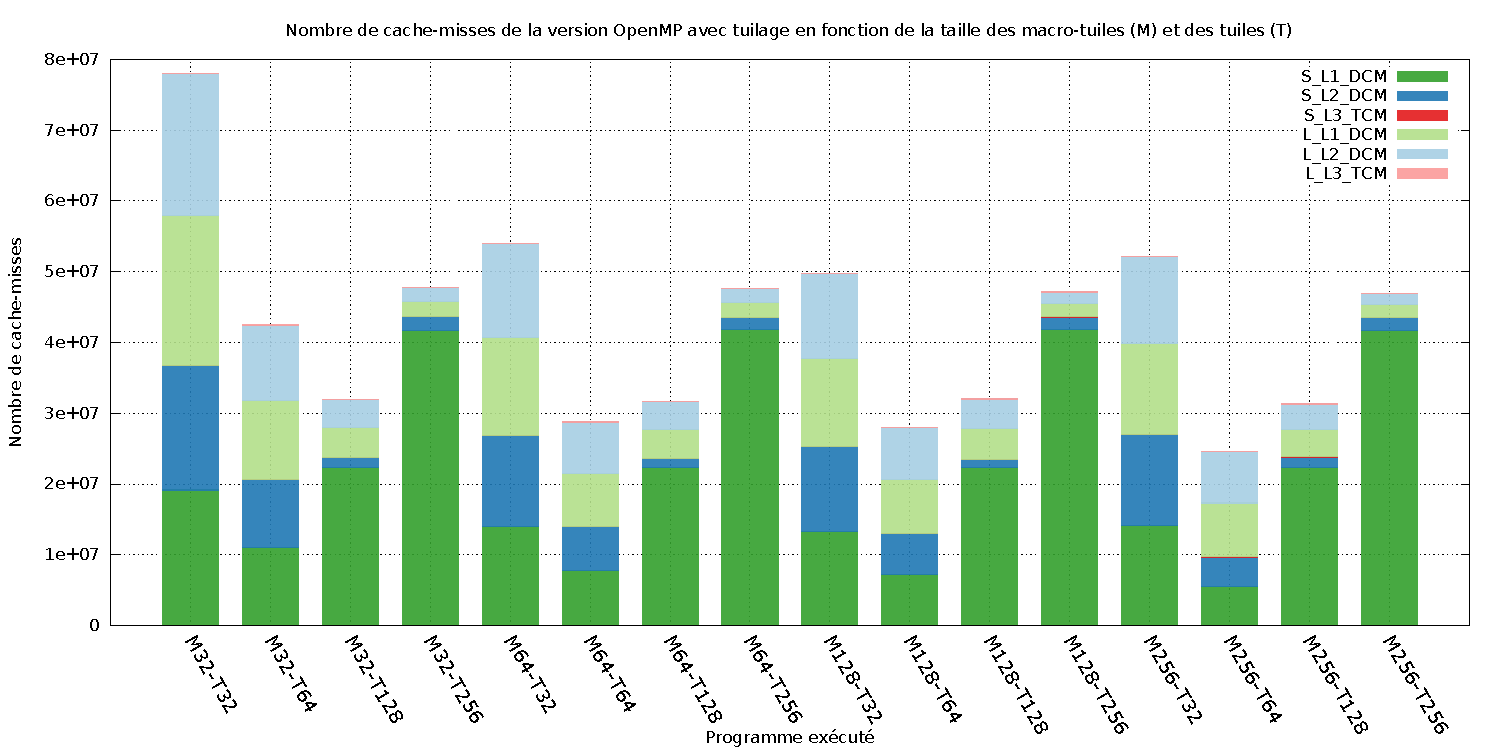
\includegraphics[width=\textwidth]{graph2.pdf}
\end{figure}

\begin{figure}[!h]
  \caption{Comparaison des performances suivant l'implantation sur un seul banc NUMA.}
  \label{graph:comp_temps_mistral10core}
  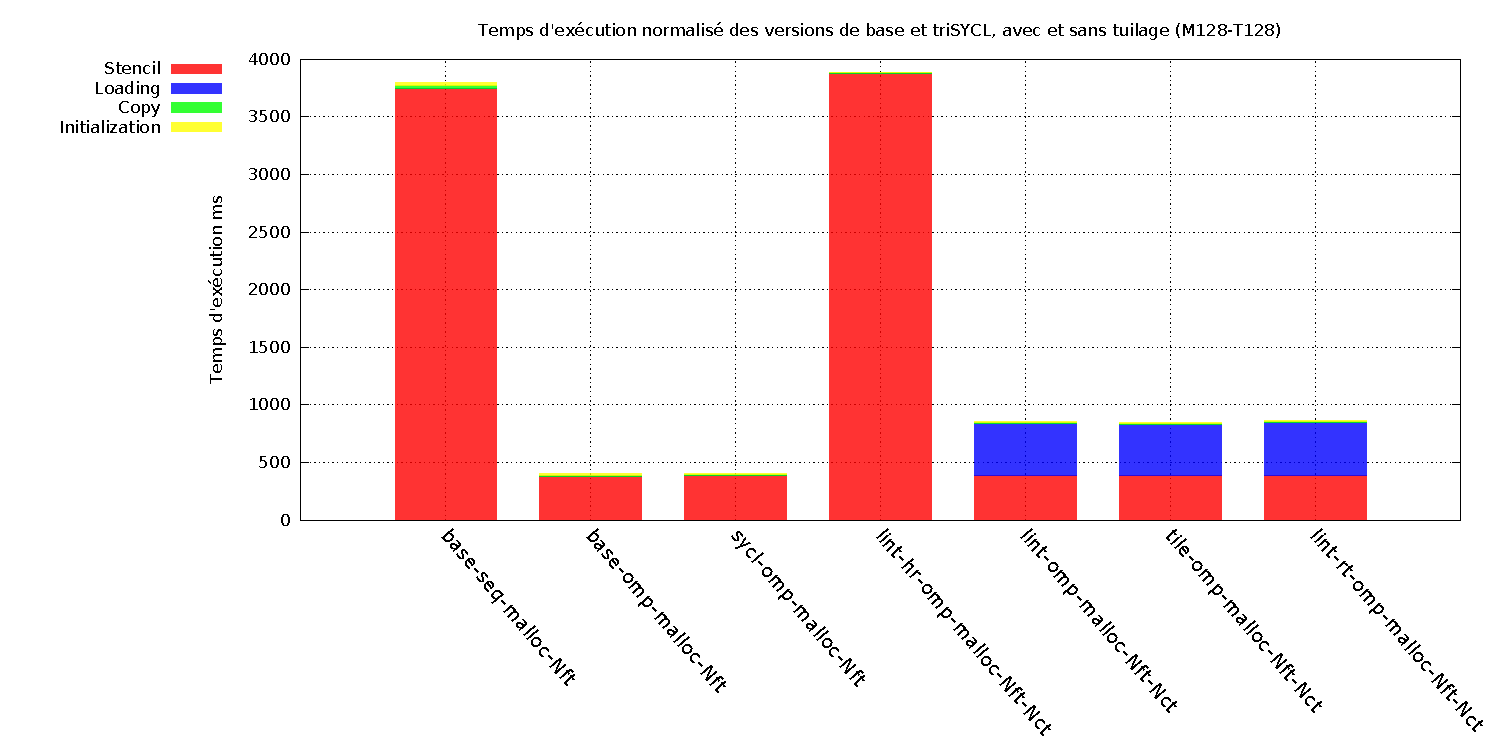
\includegraphics[width=\textwidth]{graph3.pdf}
\end{figure}

\begin{figure}[!h]
  \caption{Comparaison des performances suivant l'implantation sur deux bancs NUMA.}
  \label{graph:comp_temps_mistral20core}
  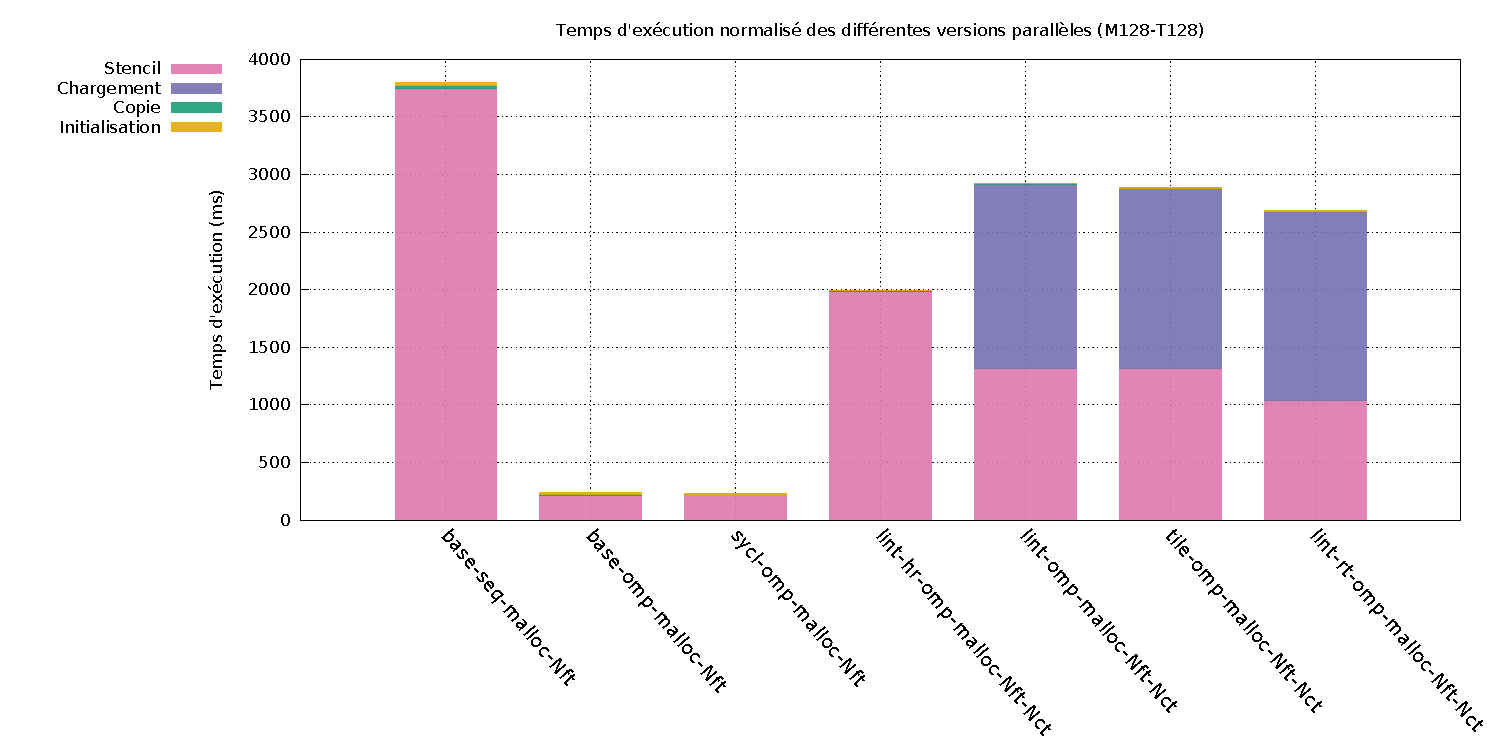
\includegraphics[width=\textwidth]{graph4.pdf}
\end{figure}

